%% cycle13_RegSnap.tex
%
%  Spitzer Space Telescope Cycle-13 Proposal Template
%
%  Use this template for Cycle-13 Regular GO and Snapshot proposals.
%  No style file is required.
%
%  Version 1.0    9 Feb 2016
%
%%%  For Spitzer proposal preparation resources please visit 
%    the proposal kit web page: 
%
%%%  http://ssc.spitzer.caltech.edu/warmmission/propkit/ 
%
%  In particular, please read the Cycle-13 Call for Proposals (CP).
%  It is the definitive document that describes the requirements
%  necessary for your proposal. 
%
%    Please address all questions regarding the proposal call
%    and observation planning to the Helpdesk at 
%
%%%  help@spitzer.caltech.edu
%
%
%
%%%%%%%%%%%%%%%%%%%%%%%%%%%%%%%%%%%%%%%%%%%%%%%%%%%%%%%%%%%%%%%%%%%%%%%%
%
%  The template begins here.  The font must be 12 point and the margins
%  must be at least 1-inch on all sides. 
%  Don't override this.  
%
% If you compile this and find that the text is "mushed up against
% the top of the page", the default paper size for your installation 
% of latex is A4.  In order to override this, do:
% > latex texfile # where the manuscript is in a file named texfile.tex
% > dvips -Ppdf -t letter -o texfile.ps texfile
% finally, to get nice (non-blurry, searchable) pdf do:
% > ps2pdf14 texfile.ps  texfile.pdf
% if you do not have ps2pdf14, please ask your sysadmin to install it.


\documentclass[letterpaper,12pt]{article}
\usepackage{epsfig}
\textwidth=6.5in
\textheight=9.5in
\topmargin=-0.75in
\oddsidemargin=0.0in
\evensidemargin=0.0in

\pagestyle{myheadings}
\usepackage{natbib}
\setlength{\bibsep}{0pt}
\newcommand{\aj}{AJ}
%\renewcommand{\aj}{AJ}
          % Astronomical Journal 
\newcommand{\araa}{ARA\&A}
%\renewcommand{\araa}{ARA\&A}
          % Annual Review of Astron and Astrophys 
%\renewcommand{\apj}{ApJ}
\newcommand{\apj}{ApJ}
          % Astrophysical Journal 
\newcommand{\apjl}{ApJ}
          % Astrophysical Journal, Letters 
\newcommand{\apjs}{ApJS}
          % Astrophysical Journal, Supplement 
%\renecwommand{\ao}{Appl.~Opt.}
\newcommand{\ao}{Appl.~Opt.}
          % Applied Optics 
\newcommand{\apss}{Ap\&SS}
          % Astrophysics and Space Science 
\newcommand{\aap}{A\&A}
          % Astronomy and Astrophysics 
\newcommand{\aapr}{A\&A~Rev.}
          % Astronomy and Astrophysics Reviews 
\newcommand{\aaps}{A\&AS}
          % Astronomy and Astrophysics, Supplement 
\newcommand{\azh}{AZh}
          % Astronomicheskii Zhurnal 
\newcommand{\baas}{BAAS}
          % Bulletin of the AAS 
\newcommand{\jrasc}{JRASC}
          % Journal of the RAS of Canada 
\newcommand{\memras}{MmRAS}
          % Memoirs of the RAS 
\newcommand{\mnras}{MNRAS}
          % Monthly Notices of the RAS 
\newcommand{\pra}{Phys.~Rev.~A}
          % Physical Review A: General Physics 
\newcommand{\prb}{Phys.~Rev.~B}
          % Physical Review B: Solid State 
\newcommand{\prc}{Phys.~Rev.~C}
          % Physical Review C 
\newcommand{\prd}{Phys.~Rev.~D}
          % Physical Review D 
\newcommand{\pre}{Phys.~Rev.~E}
          % Physical Review E 
\newcommand{\prl}{Phys.~Rev.~Lett.}
          % Physical Review Letters 
\newcommand{\pasp}{PASP}
%\renewcommand{\pasp}{PASP}
          % Publications of the ASP 
\newcommand{\pasj}{PASJ}
          % Publications of the ASJ 
\newcommand{\qjras}{QJRAS}
          % Quarterly Journal of the RAS 
\newcommand{\skytel}{S\&T}
          % Sky and Telescope 
\newcommand{\solphys}{Sol.~Phys.}
          % Solar Physics 
\newcommand{\sovast}{Soviet~Ast.}
          % Soviet Astronomy 
\newcommand{\ssr}{Space~Sci.~Rev.}
          % Space Science Reviews 
\newcommand{\zap}{ZAp}
          % Zeitschrift fuer Astrophysik 
\newcommand{\nat}{Nature}
          % Nature 
\newcommand{\iaucirc}{IAU~Circ.}
          % IAU Cirulars 
\newcommand{\icarus}{Icarus}
          % Icarus
\newcommand{\aplett}{Astrophys.~Lett.}
          % Astrophysics Letters 
\newcommand{\apspr}{Astrophys.~Space~Phys.~Res.}
          % Astrophysics Space Physics Research 
\newcommand{\bain}{Bull.~Astron.~Inst.~Netherlands}
          % Bulletin Astronomical Institute of the Netherlands 
\newcommand{\fcp}{Fund.~Cosmic~Phys.}
          % Fundamental Cosmic Physics 
\newcommand{\gca}{Geochim.~Cosmochim.~Acta}
          % Geochimica Cosmochimica Acta 
\newcommand{\grl}{Geophys.~Res.~Lett.}
%\renewcommand{\grl}{Geophys.~Res.~Lett.}
          % Geophysics Research Letters 
\newcommand{\jcp}{J.~Chem.~Phys.}
          % Journal of Chemical Physics 
\newcommand{\jgr}{J.~Geophys.~Res.}
%\renewcommand{\jgr}{J.~Geophys.~Res.}
          % Journal of Geophysics Research 
\newcommand{\jqsrt}{J.~Quant.~Spec.~Radiat.~Transf.}
          % Journal of Quantitiative Spectroscopy and Radiative Trasfer 
\newcommand{\memsai}{Mem.~Soc.~Astron.~Italiana}
          % Mem. Societa Astronomica Italiana 
\newcommand{\nphysa}{Nucl.~Phys.~A}
          % Nuclear Physics A 
\newcommand{\physrep}{Phys.~Rep.}
          % Physics Reports 
\newcommand{\physscr}{Phys.~Scr}
          % Physica Scripta 
\newcommand{\planss}{Planet.~Space~Sci.}
          % Planetary Space Science 
\newcommand{\procspie}{Proc.~SPIE}
          % Proceedings of the SPIE 


% Please update the following line with the title of your proposal
% and your Author name (with "et al." if more than two authors).

\markright{Characterizing the Dust from Disintegrating Planets, E.\ Schlawin et al.}
\pagenumbering{arabic}

\begin{document}

%\noindent {\bf Sections and Page limits:\\
%Science Plan\\
%Science Justification:  Small: 1 page; Medium: 2 pages;  Large: 3 pages; Snap $\ge$500 hr: 3 pages\\
%Technical Justification:  Small: 1 page; Medium: 1 page;  Large: 2 pages; Snap $\ge$500 hr: 2 pages\\
%Figures, Tables, References:  Small: 1 page; Medium: 2 pages;  Large: 3 pages; Snap $\ge$500 hr: 3 pages\\
%Additional Required Sections \\
%Summary of Existing Programs:  1 page\\
%Observation Summary Table:  no page limit\\
%Modification of the Proprietary Period:  no page limit\\
%Summary of Duplicate Observations:  no page limit\\
%Summary of Scheduling Constraints/ToOs:  no page limit\\}
% We'll need about 33 hr, so It's a "Medium Proposal"

\section{Science Plan}

%The Science Plan includes three parts:\newline
%
%\noindent SCIENCE JUSTIFICATION\\
%TECHNICAL JUSTIFICATION\\
%FIGURES, TABLES \& REFERENCES\\
%
%The total page limit for the Science Plan is 3 pages for small GO or Snapshot proposals 
%($<= 10$ hours), 5 pages for medium GO or Snapshot proposals (10 - 100 hours),
%8 pages for large GO or Snapshot proposals (100 - 500 hours) and 8 pages for Snapshot
%proposals $\ge$ 500 hours. Detailed page limits and descriptions of required 
%sections are provided in Chapter 5 of the Call for Proposals.\newline
%
%For joint observatory proposals one additional page per 
%joint observatory should be included to describe the 
%technical justification of the joint observations. Therefore 
%the total number of allowed pages increases by one page for 
%each joint observatory included.  

\subsection{Science Justification}

\noindent {\bf Disintegrating Bodies - A New Class of Planets}\\
The Kepler Observatory has ushered in a new era of planet discovery and characterization, and dramatically increased the inventory of known planets and planet candidates.
One of the fascinating new classes of planets uncovered by Kepler is that of disintegrating rocky bodies,
which include KIC 12557548b (hereafter shortened to KIC 1255b) \citep{rappaport} and K2-22b \citep{sanchis-ojedak2-22}.
The KIC 1255 and K2-22 systems are sufficiently bright ($K$=13.3 and $K$=11.9, respectively) for high precision Spitzer IRAC photometry.
They are also both periodic and have well-measured ephemerides that can be followed up with Spitzer.
\textbf{Disintegrating systems offer a rare opportunity to study planets that are being peeled away layer by layer}, and complement studies of white dwarfs, which are sensitive to the bulk compositions of accreted planetesimals \cite[e.g.][]{jura2003wdPollution}.
Thus far, these are the only opportunities we have for accessing different interior layers of exoplanets.
This will be the last chance for infrared characterization until the James Webb Space Telescope begins science in 2019.\newline

\noindent {\bf Particle Size and Composition}\\
The K2-22b and KIC 1255b systems show broadband flux decreases that likely comes from the scattering of dust particles -- gas absorption from atomic or ionized gas would not have enough opacity to create the large broadband transits observed by Kepler photometry \citep[0.42 $\mu$m to 0.90 $\mu$m bandpass;][]{koch2010keplerChar}.
The creation and/or destruction of dust particles cause variable transit depths, shown in Figure \ref{fig:exKeplerCurves}.
The transit depths can vary from $\sim$0\% (undetected) to 1.3\% depending on the level of disintegration activity.
The disintegration is correlated to magnetic activity on the surface of the K5 star in the KIC 1255 system \citep{kawahara2013starspots}, but this effect may be lessened by occultations of starspots by planetary debris \citep{croll2015starspots}.

The slope of the transmission spectra for these disintegrating bodies is sensitive to particle size with a steep spectral slope indicating small particle sizes and a shallow spectral slope indicating large particle sizes.
There are some indications that the spectral slope (and thus particle size) changes over time.
\citet{bochinski2015evolving} find that the slope of the KIC 1255b spectrum changes between two nights and that the spectral slope between the $u'$, $g'$ and $z'$ bands was flatter during a shallow transit than a deeper transit. 
\cite{sanchis-ojedak2-22} also find that K2-22b shows a steeper spectral slope during a deeper ($\sim 0.8\%$) event whereas a flat spectrum during a shallower ($\sim$ 0.4\% event).
Still, the particle sizes above $\sim$0.5$\mu$m as well as their composition remain unknown.

We aim to use Spitzer photometry to characterize the particle sizes of the debris to higher precision than has been achieved with ground-based optical and near-infrared data.
So far, there is only a lower limit on the particle sizes measured during medium and shallow transits.
A lower limit of $\sim$0.5$\mu$m was placed on the dust particle sizes for medium depth transits of KIC 1255b using simultaneous $K$ band (2.4$\mu$m) and Kepler broadband (0.42 to 0.90$\mu$m) photometry \citep{croll2014}.
Similarly, \citet{schlawin2016kic1255} find a lower limit of 0.5$\mu$m sized grains for olivine and pyroxene compositions using low resolution near-infrared spectroscopy (0.9 to 2.4$\mu$m) and optical photometry.
\textbf{Spitzer IRAC photometry is needed to study the large ($0.5\mu$m) dust particle escaping from KIC 1255b and K2-22b.}
No other observatory is capable of obtaining high precision light curves at wavelengths larger than 3$\mu$m, where the (1$\mu$m to 2$\mu$m) particles transition from high extinction cross sections to low extinction cross section and thus reveal their sizes.
These large particles constrain the disintegration mechanisms of these planet, such explosive volcanism versus condensation from a metal-rich vapor \citep{rappaport}.\newline

%\noindent {\bf Underlying Planet}\\
%
%Little is known about the underlying planets from which the disintegration occurs.
%For KIC 1255b, there are upper limits on the mass of 1.2 R$_{Jup}$ from radial velocity observations \citep{croll2014} and a radius of ~4600 km for an albedo of 1 \citep{vanWerkhoven2014} from the lack of secondary eclipse.
%Similarly, for K2-22b, the upper limit on the mass is 1.2 R$_{Jup}$ \citep{sanchis-ojedak2-22} from radial velocity data but this does not constrain the properties of the planet other than ruling out stellar-mass objects as causing the transit-like features.
%In the event of weak disintegration activity and small particle sizes, Spitzer photometry can put new constraints on the size of the planet \newline

\noindent {\bf Tail Geometries}\\
The K2-22 and KIC 1255 systems are interesting to compare and contrast because they display many of the same stochastic transit depth behaviors, but have different transit profiles.
KIC 1255b and K2-22b have orbital periods of 9.1 and 15.7 hours, respectively, but have about the same 2100 K equilibrium temperature because of K2-22b's  500 K cooler host star \citep{sanchis-ojedak2-22}.
The transit profile for KIC 1255b is highly asymmetric, suggesting a comet-like tail trailing the planet whereas K2-22b is more symmetric, shown in Figure \ref{fig:TransitProfiles}.
For K2-22b, the material appears to exhibiting Roche-lobe overflow onto the host star \cite{sanchis-ojedak2-22}.
We will explore the effect of particle sizes on these two different geometries for the two systems.
\newline

\noindent {\bf Transit Variability}\\
One of the great challenges of disintegrating planet systems is that the transit depths are wildly stochastic and unpredictable, as shown in Figure \ref{fig:exKeplerCurves}.
Our observing program requires that at least 3 transits be observed for a given target to ensure that sufficiently deep transits will be observed.
Table \ref{tab:probabilities} shows if 3 transits are observed for each system, there is more than a 98\% chance of observing a transit with a depth at least 0.3\%, which can place strong constraints on the size of particles escaping K2-22b and KIC 12557548b.\newline

\noindent {\bf Coordinated Simultaneous Observations}\\
It is essential to make simultaneous observations with Spitzer at shorter wavelengths in order to measure the transmission spectral energy distribution of the dust grains escaping K2-22b and KIC 1255b.
As discussed in the Science Justification, the spectral slope of the grains reveals the particle size distribution.
We therefore include only times that can be observed simultaneously with ground-based photometry.
Our team has extensive experience with ground-based observatories through Carnegie observatories, CFHT and the University of Arizona as well as a strong track record of obtaining time on telescopes for time series observations.\newline

\noindent {\bf Main Objective}\\
Aside from a few limits from ground-based observations, the particle size distribution of these disintegrating bodies is largely unknown.
Our main objective is shown in Figure \ref{fig:SizeConstraints}, where we plot the optical to infrared opacity ratio and how it constrains particle size.
\textbf{We will measure the transit depths in both the optical (using ground based data) and with Spitzer in the IRAC 3.6 $\mu$m band.
The ratio of these two bands is measures the particle sizes of escaping planet debris up to $\sim$1.5 $\mu$m.}
The particle sizes can be used to constrain the mass loss rate of the system and help distinguish mass loss mechanisms.

%We have a Cycle 24 HST proposal submitted to observe the same targets with a near-infrared grism.


%The panels have broad scientific expertise.  Include background 
%on the subject you are studying, in particular to help investigators 
%not in your sub-field understand the importance of the research. \newline

%\noindent {\bf General Advice}\\
%If you would like a step-by-step walkthrough of how to submit a
%proposal using Spot, and hints and tips for doing so, please see
%the Observation Planning Cookbook, available on the SSC website.\newline
%
%Please read the Call for Proposals (CP). It is
%the definitive document that describes the requirements
%necessary for your proposal. \newline 
%
%You must submit a PDF version of your proposal. \newline
%
%\noindent {\bf Note that there is no abstract or title or list of people
%in the Science Plan.}  The abstract and title and PI/Co-Is are part of
%the coversheet, which is all information you enter into Spot
%when you submit your proposal.  This coversheet is generated by
%the SSC for the final submission; if you want your very own
%copy, see under the ``File'' menu in the Proposal Tool in Spot.\newline
%
%Do not reduce the size of the margins or fonts.  This annoys the reviewers.
%Unusual fonts do not render on all systems.  Don't change the
%font size of the major headers --  large section header
%fonts make the proposal easier to scan. \newline
%
%Every section listed here has a purpose so please include all of them.
%Do not attach any additional material, e.g. letters of endorsement.

\clearpage

\subsection{Technical Justification}

\noindent {\bf Time Critical Requirements}\\
Our observations are \textbf{time critical} and must occur during transit so we refer to the ephemerides in Observation Summary.
Furthermore, there have been quiescent periods observed for KIC 1255b of about ~30 days in duration \citep{vanWerkhoven2014}.
We request that the transit observations are separated by 30 days to ensure that they do not fall within quiescent period where all transit depths may be shallow ($< \sim 0.2\%$ depth).
\newline

\noindent {\bf Signal To Noise}\\
Both planet systems would benefit from the long ``leaver arm'' of 4.5$\mu$m photometric measurements. However, signal to noise considerations limit the KIC 1255 observations to the 3.6 $\mu$m band.
For consistency and because there is already evidence for wavelength dependence for K2-22b at short wavelengths, we will observe both systems in the 3.6 $\mu$m band.
We used \texttt{pysynphot} with Phoenix stellar models and Simbad $K$ magnitudes to calculate a 3.6 $\mu$m IRAC flux of 1.4 mJy for KIC 1255 and 5.2 mJy for K2-22.
We plugged these values into the time series calculator, \texttt{snirac\_warm}.
For the background fluxes, we use average values provided by Spot of 0.2 MJy/sr for K2-22 and 0.06 MJy/sr for the 3.6$\mu$m band for KIC 1255.
In an optimistic case, we can obtain a SNR of 14,000 in 20 minutes of integration for K2-22 and 5,500 for 20 minutes of integration for KIC 1255.
Even when scaling down the SNR by a factor of 2 discussed in the \texttt{snirac\_warm} documentation, small transit events (0.2\% deep) are detectable at a 5.5 $\sigma$ level for KIC 1255b and 14 $\sigma$ for K2-22b.

The targets in this program are bright enough that confusion limits are not going to present an issue and any astrophysical background will be subtracted out with the aperture photometry and time series baseline. K2-22 has nearby companion star at 1.9'' that will blend the source star, but this can be accounted for using the photometry from Adaptive Optics measurements \citep{sanchis-ojedak2-22}.\newline

%This section contains the technical details for your program. 
%The Technical Justification should contain details of your planned observations, 
%descriptions of scheduling constraints, data analysis plans and a 
%description of how the technical details were validated. For proposals that 
%include generic targets or targets of opportunity, this section should also 
%include a discussion of the provenance and availability of the 
%proposed targets.\newline
%
%Note that you do NOT need to cut-and-paste the AORs into your
%proposal; you submit your proposal using Spot, and the AORs in
%the AOR window when you submit are the ones attached to your
%proposal.  If you accidentally submit the wrong ones, don't worry;
%you can update your proposal as often as you want before
%the deadline.\newline
%
%Make your plans clear by summarizing information in tables
%and using the Observation Summary Table (section 3) to your advantage.\newline
%
%Include brightness estimates 
%for your targets; for example, see the Observation Summary Table
%in section 3.  Based on those brightness estimates, include
%your estimate and justification of what kind of S/N values you
%need to accomplish your science.  Finally, include your
%assessment of background levels (based on Spot, ISSA plates,
%etc.) and explain (if necessary) how you can see your targets
%despite the background. You should include numbers from the 
%online SENS-PET (using the appropriate background setting) 
%that justify going as deeply (or as shallowly) as you have.\newline

%You should explain why you don't need to worry
%about confusion limits or saturation limits, as appropriate, or
%(alternatively) why you think you can get around these limits.\newline
\noindent {\bf Observing and Reduction Strategy}\\
We have followed the Time Series strategies suggested on the Spitzer website.
These include PCRS peakups to place the source on a detector ``sweet-spot'' that has been well characterized and calibrated.
We have included 30 minutes of dithered observations preceding the time series to help stabilize and settle the telescope prior to collecting science data.
For the science frames, we are using repeats rather than dithers because we are doing time series
monitoring and wish to place our object on the same part of the
array.

%Justify any use of low-impact Target of Opportunity observations. \newline
%
%If you have many targets, you may wish to include a separate 
%table rather than a text summary here. Organize the
%table in whatever way makes the most sense to you.   
%Please note: this table is NOT the Observation
%Summary Table described in the CP and below.  \newline
%
%You can also put information about backgrounds or expected target 
%fluxes (or both) into the Observation Summary Table (section
%3), because the Observation Summary Table does not have page
%limits.  \newline
%
%Be sure to include here a detailed assessment of duplications and 
%constraints, just {\em summaries} of which are placed in
%sections 5 and 6.\newline
Our observing team has extensive experience with high precision ground-based photometry and spectroscopy. 
We will process with time series data with these existing pipelines as well as consult with other exoplanet scientists who have analyzed secondary eclipses, transits and phase curves with the IRAC warm mission.
The many systematics present in Spitzer light curves should significantly impact our science case since the debris escaping these disintegrating planets has a much larger surface area than the atmospheres of planets typically probed with transit observations.
%
%Finally, have a detailed description of how you will handle the
%data you get, and who will do what from the list of Co-Is.  You
%might want a description of who will lead the entire effort, and
%any additional management discussion for large collaborations. 

\clearpage
\subsection{Figures, Tables \& References}

\begin{figure}
\centering
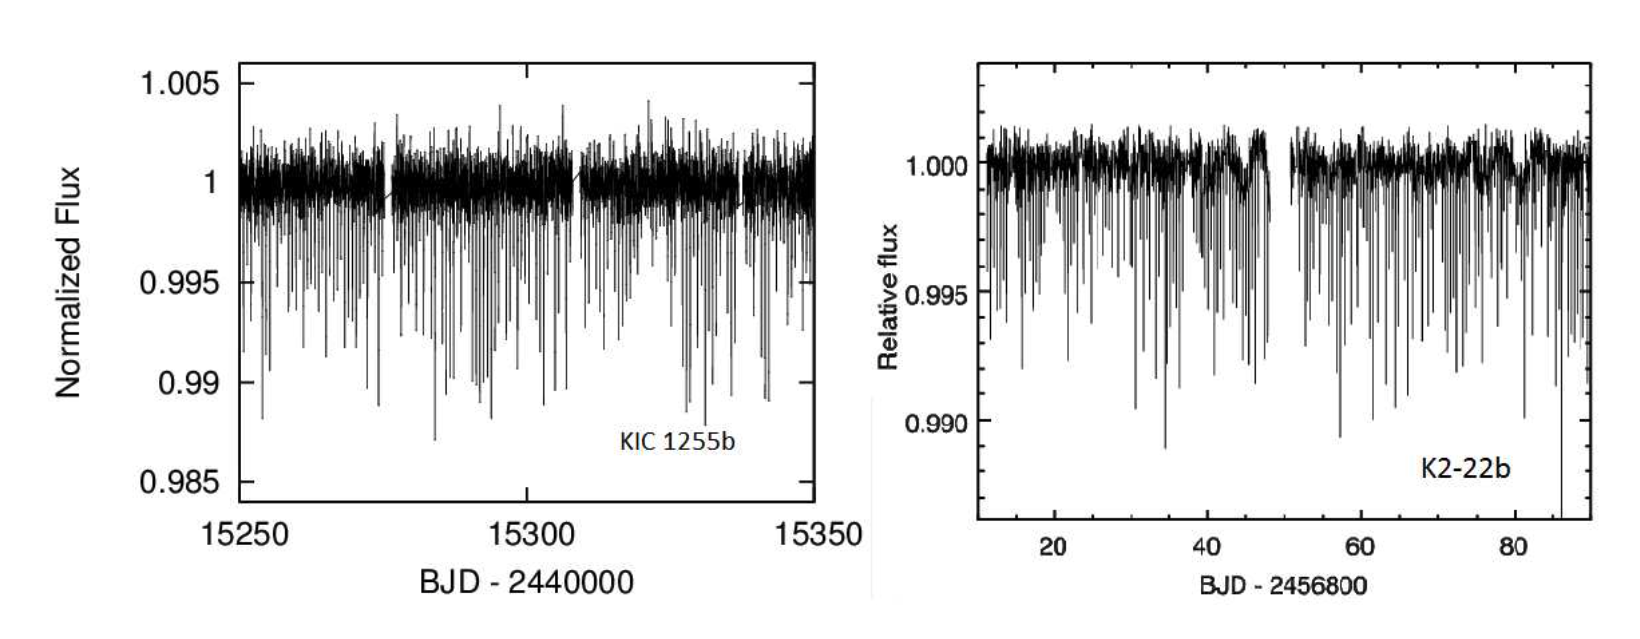
\includegraphics[width=0.9\textwidth]{kepler_lightc_variable.png}
\caption{Example lightcurves for KIC 1255b (left) and K2-22b (right) from the Kepler Observatory. The transits are periodic, but highly variable depth, suggesting that the planets are disintegrating into tails of dusty effluents.}\label{fig:exKeplerCurves}
\end{figure}

\begin{figure}
\centering
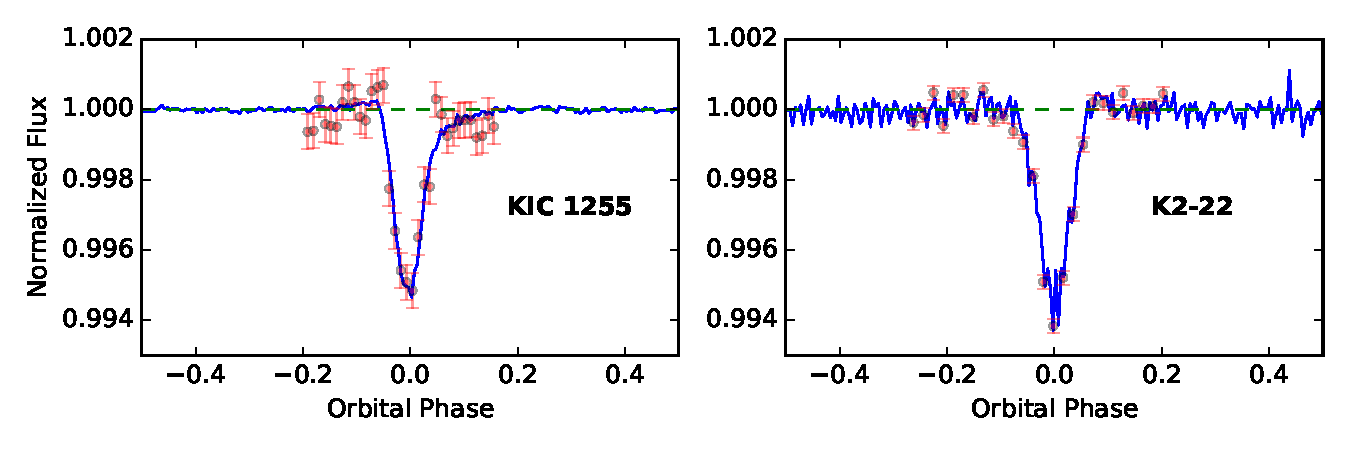
\includegraphics[width=1.0\textwidth]{transit_profiles.pdf}
\caption{Transit profiles for KIC 1255b (left) and K2-22b (right) from the Kepler Observatory phased to their respective periods of 15.7 hr and 9.1 hr. KIC 1255b has a highly asymmetric transit profile, likely coming from a comet-like tail trailing the planet at higher semi-major axes.
K2-22b is more symmetric and so it likely has both leading and trailing tails of dusty debris.
We will measure particle size distributions to contrast these two planet candidate systems.
Representative error bars are shown with twice the error predicted by \texttt{snirac\_warm} and are binned to 10 minutes for clarity.}\label{fig:TransitProfiles}
\end{figure}

\begin{figure}
\centering
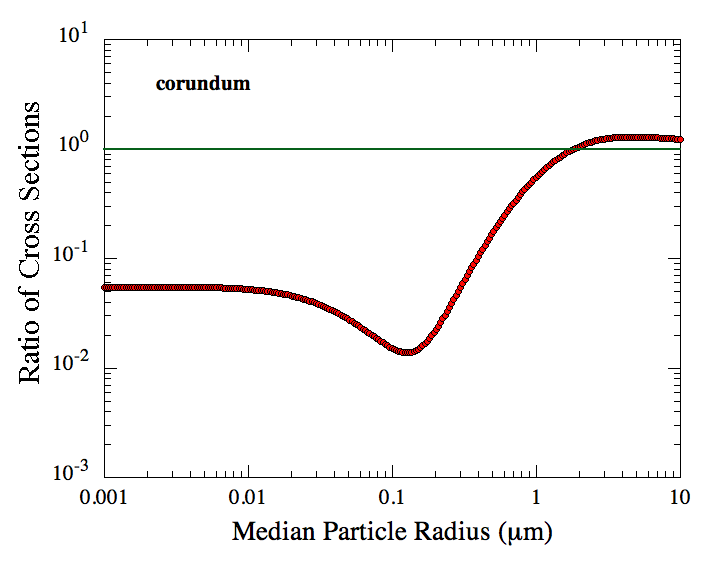
\includegraphics[width=0.55\textwidth]{particle_size_constraints.png}
\caption{The ratio between optical (0.6$\mu$m) and infrared (3.6$\mu$m) cross section (a proxy for transit depth) is plotted as a function of particle size for Corundum grains. We will measure this ratio with Spitzer 3.6$\mu$m and simultaneous ground-based photometry. \textbf{This combination of optical/infrared photometry will measure the particle sizes of dusty debris of disintegrating planets out to particle sizes of $\sim$1.5 $\mu$m for the first time.}}\label{fig:SizeConstraints}
\end{figure}

\begin{table*}[b]
\centering
%\vspace{-2.2in}
\begin{tabular}{|c | c c c| c c c|} 
\hline\hline 

	   	&     				& {\bf KIC 1255b}		&				&				& {\bf K2-22b}		&		  		\\
  $N$   	&    $\delta$ $\ge$ 0.35\%	& $\delta$ $\ge$ 0.5\%		& $\delta$ $\ge$ 0.7\%		& $\delta$ $\ge$ 0.3\%		& $\delta$ $\ge$ 0.5\%		& $\delta$ $\ge$ 0.7\%		\\
 	   	&    $P$(\%)              & $P$(\%)				& $P$(\%) 		& $P$(\%)			& $P$(\%) 		& $P$(\%)			\\
\hline 
% \multicolumn{2}{c}{KIC 1255b}\\
\hline
	1	&	98.3			& 90.6 				& 66.2			& 99.2			& 94.6			& 82.4	\\
	2	& 	84.0			& 56.8				& 22.0			& 89.5			& 68.0			& 41.0	\\
	3	& 	41.7			& 16.2				& 2.8				& 51.0			& 24.1			& 8.5		\\

\hline 
\end{tabular}
\caption{$P$ is the probability that at least $N$ of our three
transits will have a transit depth $\delta$ equal or deeper than the given values. We should have a 98.3\% and 99.2\% chance of observing one transit deep enough to 
differentiate 0.1 $\mu m$ grains from 1.0 $\mu m$ with $>$3$\sigma$ confidence
for KIC 1255b and K2-22b, respectively.}
\label{tab:probabilities}
%\vspace{0.8in}
\end{table*}



%Figures are an excellent way to convey information to your reviewers.
%Captions, tables and references may be in 10-point font.  Figures and tables 
%can be embedded within the narrative text in the Science Plan or 
%segregated into a separate section. \newline

\bibliographystyle{aasjournal}
\begingroup
\renewcommand{\section}[2]{}%
%\renewcommand{\chapter}[2]{}% for other classes
\bibliography{spitz13prop}
\endgroup


%\begin{figure}[ht]
% \begin{center}
% \epsfig{file=file1.eps, width=10cm}
%\end{center}
%\caption{Sample caption for one method of including figures.}
%\end{figure}

%\begin{figure*}
%    \centering
%    \includegraphics[width=7.5cm, angle=0]{file1.ps}
%    \includegraphics[width=7.5cm, angle=0]{file2.ps}
%\caption{Sample caption for another completely different but equivalent method of including figures.}
%\end{figure*}

\clearpage
\noindent {\bf In addition to the Science Plan, the following 1-page section is required:}

\section{Summary of Existing Programs}

%No more than one page should be used to summarize your current
%involvement as a Principal Investigator or Technical Contact on existing 
%Spitzer Space Telescope research programs. This applies to the PI and 
%key Co-Is on the proposal. The proposer should indicate the status of 
%each Spitzer GTO, GO, Legacy, DDT, Archival or Theoretical program and 
%any publications resulting from the program(s). For observing programs, 
%include the status of the data analysis effort.
%
%Proposers that are the PI/Technical contact for multiple Spitzer programs 
%are not required to provide a detailed status for every program. They 
%should provide a summary that includes the number of programs, overall 
%status (e.g. 75\% observed, 50\% data analysis complete, 20 papers published, 
%20 papers submitted, etc.) that will allow the reviewers to understand 
%the state of the programs.\newline


%PI J.\ Smith is also PI of GO-12 program xxxx, and is the TC for
%DDT program yyy.  The data for these programs have not yet been
%obtained.
%
%Co-I Q.\ Jones is the TC for GTO program zzz.  These data are
%discussed in 2013, ApJ, xxx, xxx.
%
%Co-I X.\ Kim is the PI of DDT program xxx.  These data have been
%processed and are anticipated to be submitted for publication
%this summer.\newline
\clearpage
\noindent {\bf The following sections are required but do NOT have page limits:}

\section{Observation Summary Table}\label{sec:ObsSumm}

%This section has no page limit. An observation summary table is required for all 
%proposals.  See the CP for the details of what is required. This section should not
%have any figures. The table can be tailored to your proposed observations
%but should at minimum, list each proposed observation with the position,
%integration time per array, map size (if larger than one field of view), 
%and estimated source fluxes. All of the targets submitted in the AORs 
%should be described in the Observation Summary Table.\newline

%{\bf A Perl script that parses information from the AOR file into 
%a format that can be reformatted into a table is available in the Proposal Kit.}\newline

%This table should not use a microscopic font; there are no page
%limits here, so if you need 10 pages to list all 400 sources that
%you are observing, please don't feel that they have to be listed
%in 6pt font. The table presented here is an example for the extragalactic 
%First Look Survey Field.\newline

\bigskip
\begin{tabular}{lllllcc}
\hline \\ 
Target & Position & Flux     & IRAC  & Int./ & AOR & \# of \\
Field & (J2000)   & (mJy) & Band & Pixel & Duration & AORS \\
& &  & ($\mu$m) & (secs) & (hr) & \\
\hline \\ 
KIC 12557548 & 19:23:51.9+51:30:17 & 1.4 & 3.6 & 2 & 5.9 & 3 \\
K2-22 & 11:17:55.9+02:37:09 & 3.3 & 3.6 & 2 & 5.0 & 3 \\
\multicolumn{7}{c}{Each set of AORs is repeated 3 times} \\
\hline \\
\end{tabular}


There are 33 hrs total requested for this observing program.\newline

%If joint time with HST or Chandra is also proposed, please summarize 
%here how many orbits or kiloseconds of time are requested.


\section{Modification of the Proprietary Period}

%This section has no page limit. The default proprietary period for General 
%Observer and Snapshot programs $< 500$ hours is 365 days. 
%Please specify any requested reduction in this proprietary period in this section.
%The default proprietary period for Snapshot programs $\ge$ 500 hours is zero days.
%A maximum of 90 days can be requested and should be justified here.
We request the standard proprietary period of 365 days.

\section{Summary of Duplicate Observations}

%This section has no page limit. {\it Briefly} summarize the justification for 
%any proposed duplicate observation. The details should have been provided in the
%Science Plan.  Even if there are no duplicates, note this. Leopard should be 
%used to find any duplications, including observations that used Instrument
%Engineering Requests (IERs), since such observations will not
%show up in Spot searches. More information can be found in the
%Leopard User's Guide.\newline

There are two programs that include imaging of the targets in this proposal -- Program 10067 (PI M. Werner) and Program 11026 (PI M. Werner).
Neither of these previous programs is a transit/time series observation that can be used to extract information about the planet or their debris when going in front of the host stars, as discussed in the Science Plan.
Therefore, this program is not a duplicate observation.

%\noindent Example: 
%
%A search using Leopard of the ROC reveals a handful of apparent
%duplications with pid xxx (AOR label ``IRAC-0000''), yyy (all
%AORs), and zzz (AOR label ``IRAC-1234'').  We believe none of
%these are true duplications; see Science Plan for further discussion.  \newline
%
%\noindent or: \newline
%
%\noindent There are no duplicate observations.


\section{Summary of Scheduling Constraints/ToOs}

%This section has no page limit. Briefly summarize the justification for 
%any proposed scheduling constraints. 
%Also provide a summary of any ToO scheduling issues. 
%The details should have been provided in the Science Plan. Even if there 
%are no constraints or ToOs, note this.\newline

These observations are \textbf{time critical} and need to take place when K2-22b and KIC 1255b cross in front of their host stars.
We provide an ephemeris with our time constraints that can be observed with simultaneous ground-based observations.
Furthermore, we request that the observations of each planet system are spaced by at least 20 days to avoid falling into a weaker period observed for KIC 12557548 \citep{vanWerkhoven2014}.

%\noindent Example:
%
%We have placed a loose group-within constraint, spanning 10 days,
%on our three AORs that cover the extended target XXX to 
%minimize field rotation in the large map that will be produced by the AORs.\newline
%
%\noindent or:\noindent 
%
%We will be requesting 1 low-impact ToO and we have indicated this in the 
%AORs.  We anticipate one new comet to be discovered this year that meets 
%our criteria as discussed in the Science Plan.\newline
%
%\noindent or:
%
%There are no scheduling constraints or ToOs in this program.

\end{document}

